\documentclass{beamer}
\usepackage[utf8]{inputenc}
\usepackage{graphicx}
\usepackage{tikz}
\usetikzlibrary{arrows, positioning, shapes.geometric}
\usepackage{listings}
\lstdefinestyle{MyPythonStyle}
{
    language=Python,
    basicstyle=\footnotesize,
    numbers=left,
    stepnumber=1,
    showstringspaces=false,
    tabsize=1,
    breaklines=true,
    breakatwhitespace=false,
}
\newcommand{\NonPrivateNetflix}{\begin{tabular}{lllll}
\; & \rotatebox[origin=r]{270}{Titanic} & \rotatebox[origin=r]{270}{Date} & \rotatebox[origin=r]{270}{The Notebook} & \rotatebox[origin=r]{270}{Date} \\
Jordan & 8.5 & 1/17 & 7.5 & 3/20 \\
Jean & 6 & 3/5 & 5 & 3/7 \\
Scott & 2 & 1/21 & 9 & 2/26 \\
Serena & 4.5 & 4/5 & 9 & 3/7 \\
\end{tabular}}
\newcommand{\PrivateNetflix}{\begin{tabular}{lllll}
\; & \rotatebox[origin=r]{270}{Titanic} & \rotatebox[origin=r]{270}{Date} & \rotatebox[origin=r]{270}{The Notebook} & \rotatebox[origin=r]{270}{Date} \\
User 1 & 8.5 & 1/17 & 7.5 & 3/20 \\
User 2 & 6 & 3/5 & 5 & 3/7 \\
User 3 & 2 & 1/21 & 9 & 2/26 \\
User 4 & 4.5 & 4/5 & 9 & 3/7 \\
\end{tabular}}
\newcommand{\NonPrivateNetflixA}{\begin{tabular}{lllll}
Jordan & 8.5 & 1/17 & 7.5 & 3/20 \\
Jean & 6 & 3/5 & 5 & 3/7 \\
Scott & 2 & 1/21 & 9 & 2/26 \\
Serena & 4.5 & 4/5 & 9 & 3/7 \\
\end{tabular}}
\newcommand{\PrivateNetflixA}{\begin{tabular}{lllll}
User 1 & 8.5 & 1/17 & 7.5 & 3/20 \\
User 2 & 6 & 3/5 & 5 & 3/7 \\
User 3 & 2 & 1/21 & 9 & 2/26 \\
User 4 & 4.5 & 4/5 & 9 & 3/7 \\
\end{tabular}}
\newcommand{\Noise}{\begin{tabular}{lllll}
\qquad & 0.3 & 1.5 & -1.1 & 2.3 \\
\qquad & -0.1 & 0.3 & -0.2 & -0.7 \\
\qquad & 0.0 & -2.4 & 0.9 & -0.9 \\
\qquad & -0.2 & 1.2 & 0.4 & 1.1 \\
\end{tabular}}
\newcommand{\PrivatePrivateNetflix}{\begin{tabular}{lllll}
User 1 & 8.0 & 1/19 & 6.5 & 3/22 \\
User 2 & 6 & 3/5 & 5 & 3/6 \\
User 3 & 2 & 1/19 & 10 & 2/25 \\
User 4 & 4.5 & 4/6 & 9.5 & 3/8 \\
\end{tabular}}
\newcommand{\NonPrivateNetflixB}{\begin{tabular}{lllll}
Jordan & 8.5 & 1/17 & 7.5 & 3/20 \\
Jean & 6 & 3/5 & 5 & 3/7 \\
Scott & 2 & 1/21 & 9 & 2/26 \\
Serena & 8.5 & 4/6 & 3 & 1/20 \\
\end{tabular}}
\newcommand{\PrivateNetflixB}{\begin{tabular}{lllll}
User 1 & 8.5 & 1/17 & 7.5 & 3/20 \\
User 2 & 6 & 3/5 & 5 & 3/7 \\
User 3 & 2 & 1/21 & 9 & 2/26 \\
User 4 & 8.5 & 4/6 & 3 & 1/20 \\
\end{tabular}}
\title{Automatic, Fine-Grained Algorithmic Choice for Differential Privacy}
\author{Jacob Imola (Advisor: Jean Yang)}
\institute{Carnegie Mellon University}
\date{2017}

\begin{document}
\frame{\titlepage}

\begin{frame}{Motivation}
Netflix wants to anonymize database and release it:
\begin{center}
\NonPrivateNetflix
\end{center}
\end{frame}

\begin{frame}{Motivation}
Just cross out names!
\begin{center}
\PrivateNetflix
\end{center}
Months later...
\end{frame}

\begin{frame}{Motivation}
\begin{columns}
\begin{column}{0.5\textwidth}
Netflix
\end{column}
\begin{column}{0.5\textwidth}
IMDB
\end{column}
\end{columns}
\vspace{1em}
\begin{columns}
\begin{column}{0.5\textwidth}
\PrivateNetflix
\end{column}
\begin{column}{0.5\textwidth}
\begin{tabular}{|p{5cm}|}
\hline
Scott on 1/22: \\
\quad (1.5/5) Titanic was terrible! \\ \hline
\end{tabular}
\begin{tabular}{|p{5cm}|}
\hline
Jordan on 1/20: \\
\quad (4.0/5) Enjoyed Titanic! \\ \hline
\end{tabular}
\begin{tabular}{|p{5cm}|}
\hline
Jean on 3/6: \\
\quad (2.0/5) The Notebook was pretty overrated :/ \\ \hline
\end{tabular}
\end{column}
\end{columns}
\vspace{1em}
\alert{Netflix promised that all movie ratings would be protected!}
\end{frame}
\begin{frame}{Differential Privacy}
\begin{block}{Definition}
For all $D$ and $D'$ differing in 1 row: $P$ is $\epsilon$-DP if $\Pr(P(D) = O) < e^\epsilon \Pr(P(D') = O)$ for all $O$.
\end{block}
	\[P\underbrace{\left(\resizebox{0.3\textwidth}{!}{\NonPrivateNetflixA}\right)}_D = \underbrace{\resizebox{0.3\textwidth}{!}{\PrivateNetflixA}}_O\]
	\[P\underbrace{\left(\resizebox{0.3\textwidth}{!}{\NonPrivateNetflixB}\right)}_{D'} = \underbrace{\resizebox{0.3\textwidth}{!}{\PrivateNetflixB}}_{O'}\]
Violation: $\Pr(P(D) = O) = 1$ and $\Pr(P(D') = O) = 0$
\end{frame}
\begin{frame}{Example}
\begin{center}
A representation change
\begin{tikzpicture}
	\node[] (I) {\resizebox{0.3\textwidth}{!}{\PrivateNetflixA}};
	\node [right=1em of I] (arrow) {$\rightarrow$};
	\node [right=1em of arrow] (out) {\includegraphics[scale=0.2]{hist_graphs/I1.png}};
\end{tikzpicture}
\end{center}
\end{frame}

\begin{frame}{Example}
Method 1
\begin{center}
\begin{tikzpicture}
	\tikzset{block/.style= {draw, rectangle, align=center,minimum width=2cm,minimum height=2cm}, empty/.style= {align=center}}
	\node [empty]  (I1) {\includegraphics[scale=0.2]{hist_graphs/I1.png}};
	\node [empty, above=-0.5em of I1] (Lab1) {$D$};
	\node [empty, right=1em of I1] (plus1) {+};
	\node [empty, right=1em of plus1] (N1) {\includegraphics[scale=0.2]{hist_graphs/N1.png}};
	\node [empty, above=-0.5em of N1] (Noise1) {Noise};
	\node [empty, right=1em of N1] (equals1) {=};
	\node [empty, right=1em of equals1] (ans1) {\includegraphics[scale=0.2]{hist_graphs/A1.png}};
	\node [empty, above=-0.5em of ans1] (Output1) {$O$};
	\node [empty, below=1em of I1]  (I2) {\resizebox{0.3\textwidth}{!}{\PrivateNetflixA}};
	\node [empty, below=1em of N1] (N2) {\resizebox{0.3\textwidth}{!}{\Noise}};
	\node [empty, below=1em of ans1] (ans2) {\resizebox{0.3\textwidth}{!}{\PrivatePrivateNetflix}};
\end{tikzpicture}
\end{center}

\end{frame}

\begin{frame}{Example}
Method 1
\begin{center}
\begin{tikzpicture}
	\tikzset{block/.style= {draw, rectangle, align=center,minimum width=2cm,minimum height=2cm}, empty/.style= {align=center}}
	\node [empty]  (I1) {\includegraphics[scale=0.2]{hist_graphs/I1.png}};
	\node [empty, above=-0.5em of I1] (Lab1) {$D$};
	\node [empty, right=1em of I1] (plus1) {+};
	\node [empty, right=1em of plus1] (N1) {\includegraphics[scale=0.2]{hist_graphs/N1.png}};
	\node [empty, above=-0.5em of N1] (Noise1) {Noise};
	\node [empty, right=1em of N1] (equals1) {=};
	\node [empty, right=1em of equals1] (ans1) {\includegraphics[scale=0.2]{hist_graphs/A1.png}};
	\node [empty, above=-0.5em of ans1] (Output1) {$O$};
	\node [empty, below=1em of I1]  (I2) {\includegraphics[scale=0.2]{hist_graphs/I2.png}};
	\node [empty, above=-0.5em of I2] (Lab2) {$D'$};
	\node [empty, right=1em of I2] (plus2) {+};
	\node [empty, right=1em of plus2] (N2) {\includegraphics[scale=0.2]{hist_graphs/N2.png}};
	\node [empty, above=-0.5em of N2] (Noise2) {Noise};
	\node [empty, right=1em of N2] (equals2) {=};
	\node [empty, right=1em of equals2] (ans2) {\includegraphics[scale=0.2]{hist_graphs/A2.png}};
	\node [empty, above=-0.5em of ans2] (Output2) {$O'$};
\end{tikzpicture}
\end{center}
$\Pr(P(D) = O) \approx 10^{-8} \qquad \Pr(P(D') = O) \approx 2\times 10^{-9}$

Seeing $O$, attacker cannot distinguish $D$ and $D'$.
\end{frame}

\begin{frame}{Example}
Method Two
\begin{itemize}
\item Sum into 4 buckets, add noise, divide by 4
\end{itemize}
\begin{center}
\begin{tikzpicture}
	\tikzset{block/.style= {draw, rectangle, align=center,minimum width=2cm,minimum height=2cm}, empty/.style= {align=center}}
	\node [empty]  (I1) {\includegraphics[scale=0.2]{hist_graphs/I1.png}};
	\node [empty, above=-0.5em of I1] (Lab1) {$D$};
	\node [empty, right=1em of I1] (plus1) {$\rightarrow$};
	\node [empty, right=1em of plus1] (N1) {\includegraphics[scale=0.2]{hist_graphs/I3.png}};
	\node [empty, above=-0.5em of N1] (Noise1) {Avg};
	\node [empty, right=1em of N1] (equals1) {+Noise};
	\node [empty, right=1em of equals1] (ans1) {\includegraphics[scale=0.2]{hist_graphs/A3.png}};
	\node [empty, above=-0.5em of ans1] (Output1) {$O$};
	\node [empty, below=1em of I1]  (I2) {\includegraphics[scale=0.2]{hist_graphs/I2.png}};
	\node [empty, above=-0.5em of I2] (Lab2) {$D'$};
	\node [empty, right=1em of I2] (plus2) {$\rightarrow$};
	\node [empty, right=1em of plus2] (N2) {\includegraphics[scale=0.2]{hist_graphs/I4.png}};
	\node [empty, above=-0.5em of N2] (Noise2) {Avg};
	\node [empty, right=1em of N2] (equals2) {+Noise};
	\node [empty, right=1em of equals2] (ans2) {\includegraphics[scale=0.2]{hist_graphs/A4.png}};
	\node [empty, above=-0.5em of ans2] (Output2) {$O'$};
\end{tikzpicture}
\end{center}
\end{frame}

\begin{frame}{Example}
Which is better?
\begin{center}
\begin{tikzpicture}
	\tikzset{block/.style= {draw, rectangle, align=center,minimum width=2cm,minimum height=2cm}, empty/.style= {align=center}}
	\node [] (input) {\includegraphics[scale=0.2]{hist_graphs/I1.png}};
	\node [rectangle, draw=red, right=1em of input]  (I1) {\includegraphics[scale=0.2]{hist_graphs/A1.png}};
	\node [above=-0.5em of input] (In) {$D_1$};
	\node [empty, right=1em of I1] (plus1) {vs.};
	\node [empty, right=1em of plus1] (N1) {\includegraphics[scale=0.2]{hist_graphs/A3.png}};
	\node [above=-0.5em of I1] {Alg1};
	\node [above=-0.5em of N1] {Alg2};
	\node [below=1em of input] (input2) {\includegraphics[scale=0.2]{hist_graphs/It.png}};
	\node [right=1em of input2]  (I2) {\includegraphics[scale=0.2]{hist_graphs/Ot.png}};
	\node [above=-0.5em of input2] (In2) {$D_2$};
	\node [empty, right=1em of I2] (plus2) {vs.};
	\node [rectangle, draw=red, right=1em of plus2] (N2) {\includegraphics[scale=0.2]{hist_graphs/Ot2.png}};
	\node [above=-0.5em of I2] {Alg1};
	\node [above=-0.5em of N2] {Alg2};
\end{tikzpicture}
\end{center}
DP complicates algorithm analysis due to noise, makes algorithm deployment hard.
\end{frame}
\begin{frame}[fragile]\frametitle{Vision}
Task: Remove burden of DP algorithm analysis.
\begin{enumerate}
\item \textbf{Correctness} Differential privacy is never violated. 
\item \textbf{Generalizability} Works on arbitrary code.
\item \textbf{Performance} Makes choice ``close enough'' to optimal.
\end{enumerate}
Solution: A programming language (Jostle)!

Represent any choice with \texttt{ChoiceMaker} construct.
\begin{lstlisting}[style=MyPythonStyle]
answerHistQueries = MkChoiceMaker among {Alg1, Alg2}
answers = answerHistQueries(data, queries)
\end{lstlisting}
\end{frame}

\begin{frame}{Note on performance}
\includegraphics[scale=0.7]{hist_graphs/Perf.png}
\end{frame}

\begin{frame}{Note on performance}
\includegraphics[scale=0.7]{hist_graphs/regret.png}
\end{frame}

\begin{frame}[fragile]\frametitle{Challenges}
What's hard about writing this code?
\begin{lstlisting}[style=MyPythonStyle]
answerHistQueries = MkChoiceMaker among {Alg1, Alg2}
answers = answerHistQueries(data, queries)
\end{lstlisting}
\begin{center}
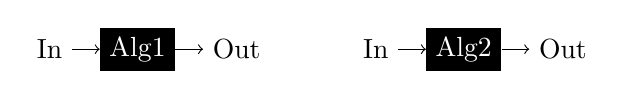
\begin{tikzpicture}
\node [align=center] (In1) {In};
\node [right=1em of In1, align=center, rectangle, fill=black, text=white] (alg1) {Alg1};
\node [right=1em of alg1, align=center] (Out1) {Out};
\draw[->] (In1) -- (alg1);
\draw[->] (alg1) -- (Out1);
\node [align=center, right=3em of Out1] (In2) {In};
\node [right=1em of In2, align=center, rectangle, fill=black, text=white] (alg2) {Alg2};
\node [right=1em of alg2, align=center] (Out2) {Out};
\draw[->] (In2) -- (alg2);
\draw[->] (alg2) -- (Out2);
\end{tikzpicture}
\end{center}
\begin{center}
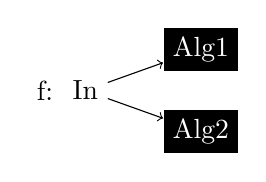
\begin{tikzpicture}
\node [align=center] (func) {f:};
\node [align=center, right=0em of func] (pairs) {In};
\node [align=center, above right=0em and 2em of pairs, rectangle, fill=black, text=white] (alg1) {Alg1};
\draw[->] (pairs) -- (alg1);
\node [align=center, below right=0em and 2em of pairs, rectangle, fill=black, text=white] (alg2) {Alg2};
\draw[->] (pairs) -- (alg2);
\end{tikzpicture}
\end{center}
\begin{itemize}
\item Generality $\implies$ Alg1, Alg2 are black boxes.
\item Approach: Meta-machine learning: $f: DB \rightarrow Alg$
\item Difficult---data science cannot be automated well.
\end{itemize}
\end{frame}

\begin{frame}{Existing Work}
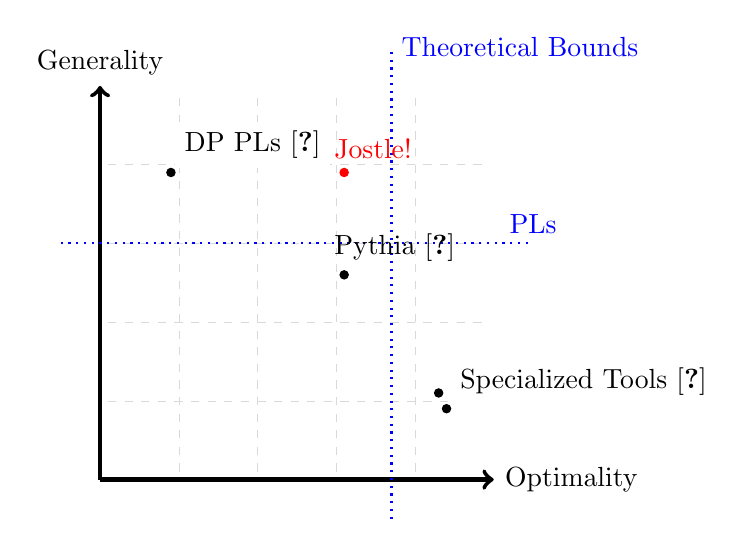
\begin{tikzpicture}
\draw[help lines, color=gray!30, dashed] (0.1,0.1) grid (4.9,4.9);
\draw[->,ultra thick] (0,0)--(5,0) node[right]{Optimality};
\draw[->,ultra thick] (0,0)--(0,5) node[above]{Generality};
\draw[dotted,thick,blue] (3.7,-0.5)--(3.7,5.5) node[anchor=west,blue] {Theoretical Bounds};
\draw[dotted,thick,blue] (-0.5,3.0)--(5.5,3.0) node[anchor=south,blue] {PLs};
\filldraw (4.3,1.1) circle[radius=1.5pt];
\node [above right=-0.5pt of {(4.4,0.9)}, outer sep=2pt, fill=white] {Specialized Tools \cite{Chaudhuri:2013}};
\filldraw (4.4,0.9) circle[radius=1.5pt];
%\node [below right=-0.5pt of {(4.4, 0.9)}, outer sep=2pt, fill=white] {1};
\filldraw (3.1, 2.6) circle[radius=1.5pt];
\node [above right=-0.5pt of {(2.8, 2.6)}, outer sep=2pt] {Pythia \cite{Kotsogiannis:2017}};
\filldraw[red] (3.1, 3.9) circle[radius=1.5pt]; 
\node [red, above right=-0.5pt of {(2.8, 3.9)}, outer sep=2pt] {Jostle!};
\filldraw[black] (0.9, 3.9) circle[radius=1.5pt];
\node [above right=-0.5pt of {(0.9, 3.9)}, outer sep=2pt, fill=white] {DP PLs \cite{McSherry:2010}};
\end{tikzpicture}
\end{frame}

\begin{frame}{Solution Overview}
\begin{itemize}
\item Metafeatures modeled after data science approach
\item $f: DB\rightarrow Alg$ becomes $f: \mathcal{X} \rightarrow Alg$.
\end{itemize}
\begin{center}
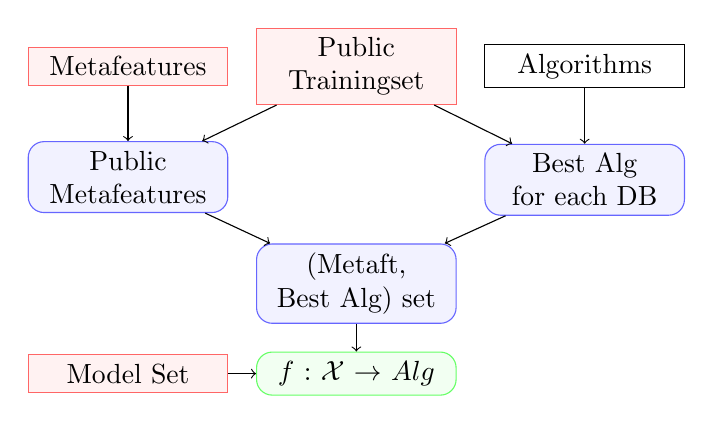
\begin{tikzpicture}
\tikzset{block/.style={rectangle, align=center,text width=2.3cm, fill=red!5, draw=red!60},
		action/.style={rectangle, align=center,text width=2.3cm, fill=blue!5, draw=blue!60, rounded corners=2mm},
		answer/.style={rectangle, align=center,text width=2.3cm, fill=green!5, draw=green!60, rounded corners=2mm},
		blank/.style={rectangle, draw, align=center,text width=2.3cm}}
\node[block] (MF) {Metafeatures};
\node[block, right=1em of MF] (PT) {Public Trainingset};
\node[blank, right=1em of PT] (Ch) {Algorithms};
\node[action, below=2em of MF] (PM) {Public Metafeatures};
\draw[->] (MF) -- (PM);
\draw[->] (PT) -- (PM);
\node[action, below=2em of Ch] (BA) {Best Alg for each DB};
\draw[->] (PT) -- (BA);
\draw[->] (Ch) -- (BA);
\node[action, below=5em of PT] (MPT) {(Metaft, Best Alg) set};
\draw[->] (BA) -- (MPT);
\draw[->] (PM) -- (MPT);
\node[answer, below=1em of MPT] (CM) {$f: \mathcal{X} \rightarrow Alg$};
\node[block, left=1em of CM] (Model) {Model Set};
\draw[->] (MPT) -- (CM);
\draw[->] (Model) -- (CM);
\end{tikzpicture}
\end{center}
Important: Trainingset must have lots of DB's for training!
\end{frame}
\begin{frame}[fragile]{Solution Overview}
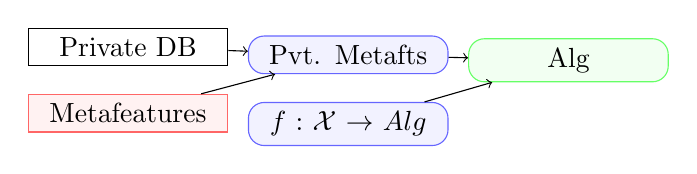
\begin{tikzpicture}
\tikzset{block/.style={rectangle, align=center,text width=2.3cm, fill=red!5, draw=red!60},
		action/.style={rectangle, align=center,text width=2.3cm, fill=blue!5, draw=blue!60, rounded corners=2mm},
		answer/.style={rectangle, align=center,text width=2.3cm, fill=green!5, draw=green!60, rounded corners=2mm},
		blank/.style={rectangle, draw, align=center,text width=2.3cm}}
\node[blank] (PDB) {Private DB};
\node[block, below=1em of PDB] (MF) {Metafeatures};
\node[action, above right=1em of MF] (PMF) {Pvt. Metafts};
\draw[->] (MF) -- (PMF);
\draw[->] (PDB) -- (PMF);
\node[action, below=1em of PMF] (CM) {$f: \mathcal{X} \rightarrow Alg$};
\node[answer, above right=1em of CM] (Alg) {Alg};
\draw[->] (PMF) -- (Alg);
\draw[->] (CM) -- (Alg);
\end{tikzpicture}
\vspace{1em}
\begin{lstlisting}[style=MyPythonStyle]
answerHistQueries = 
MkChoiceMaker among {Alg1, Alg2}
	informed by {dbSize, dbNumRows}
	modeled by LinearModel with ErrorFunc
	trained on TrainingSet}

answers = answerHistQueries(data, queries)
\end{lstlisting}
\end{frame}

\begin{frame}{Experimental Setup}
\begin{itemize}
\item \textbf{Algorithms} Stopping Criteria for Private Decision Trees.
\item \textbf{Metafeatures} DB size, epsilon, domain size.
\item \textbf{Classification} Linear Classifiers
\item \textbf{Training Set} 
\begin{enumerate}
\item 300 real DB snapshots, 100 real DB snapshots
\item 300 synth. DB snapshots, 100 synth. DB snapshots
\end{enumerate}
\end{itemize}
\begin{center}
\includegraphics[scale=0.35]{DTreeStopping}
\end{center}
\end{frame}

\begin{frame}{Results}
\begin{center}
\includegraphics[scale=0.6]{Results}
\end{center}
Always possible to have similar test DB in training DB set?
\end{frame}

\begin{frame}{Conclusion}
\begin{itemize}
\item Performs as well as Pythia \cite{Kotsogiannis:2017} with same expressiveness as PINQ \cite{McSherry:2010}.
\item Only as good as how well the programmer frames the ML.
\item Future work: Better optimization for multiple ChoiceMakers. Static analysis (open black boxes).
\end{itemize}
\begin{center}
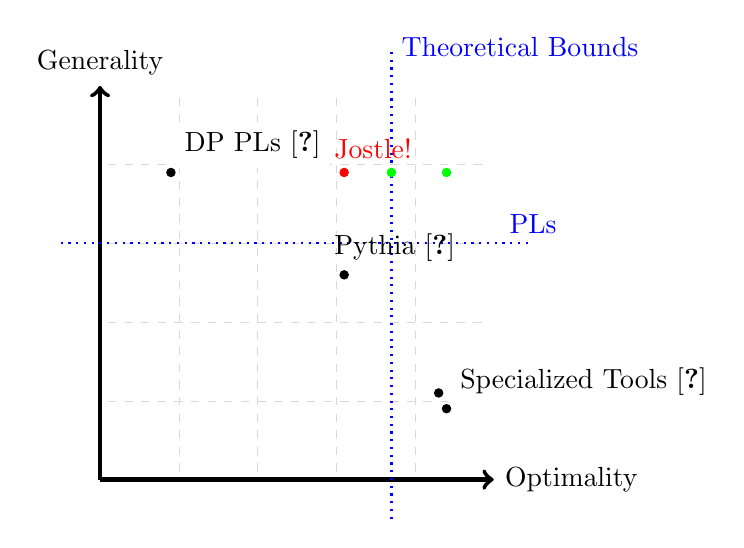
\begin{tikzpicture}
\draw[help lines, color=gray!30, dashed] (0.1,0.1) grid (4.9,4.9);
\draw[->,ultra thick] (0,0)--(5,0) node[right]{Optimality};
\draw[->,ultra thick] (0,0)--(0,5) node[above]{Generality};
\draw[dotted,thick,blue] (3.7,-0.5)--(3.7,5.5) node[anchor=west,blue] {Theoretical Bounds};
\draw[dotted,thick,blue] (-0.5,3.0)--(5.5,3.0) node[anchor=south,blue] {PLs};
\filldraw (4.3,1.1) circle[radius=1.5pt];
\node [above right=-0.5pt of {(4.4,0.9)}, outer sep=2pt, fill=white] {Specialized Tools \cite{Chaudhuri:2013}};
\filldraw (4.4,0.9) circle[radius=1.5pt];
%\node [below right=-0.5pt of {(4.4, 0.9)}, outer sep=2pt, fill=white] {1};
\filldraw (3.1, 2.6) circle[radius=1.5pt];
\node [above right=-0.5pt of {(2.8, 2.6)}, outer sep=2pt] {Pythia \cite{Kotsogiannis:2017}};
\filldraw[red] (3.1, 3.9) circle[radius=1.5pt]; 
\node [red, above right=-0.5pt of {(2.8, 3.9)}, outer sep=2pt] {Jostle!};
\filldraw[black] (0.9, 3.9) circle[radius=1.5pt];
\node [above right=-0.5pt of {(0.9, 3.9)}, outer sep=2pt, fill=white] {DP PLs \cite{McSherry:2010}};
\filldraw[green] (3.7, 3.9) circle[radius=1.5pt];
\filldraw[green] (4.4, 3.9) circle[radius=1.5pt];
\end{tikzpicture}
\end{center}
\end{frame}

\begin{frame}
\frametitle{References}
\bibliographystyle{plain}
\bibliography{Thesis.bib}
\end{frame}
\end{document}